\documentclass[tikz,border=12pt]{standalone}
\usepackage{tikz}

\definecolor{fairblue}{RGB}{33, 102, 172}
\definecolor{fairmidblue}{RGB}{103, 169, 207}
\definecolor{fairlight}{RGB}{247, 247, 247}
\definecolor{fairmidred}{RGB}{239, 138, 98}
\definecolor{fairred}{RGB}{178, 24, 43}
\definecolor{darkgray}{RGB}{60, 60, 60}
\definecolor{lightgrid}{RGB}{230, 230, 230}

\begin{document}
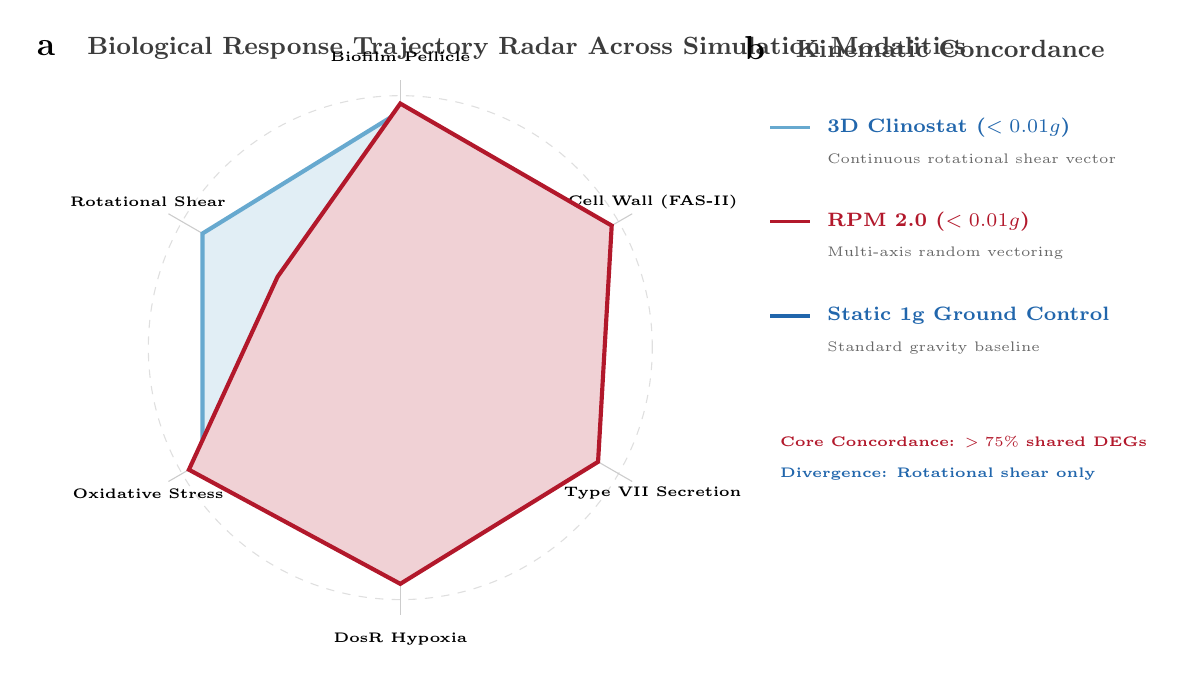
\begin{tikzpicture}[font=\sffamily]
  % Panel a: Radar Plot
  \node[font=\large\bfseries] at (0, 7.8) {a};
  \node[anchor=west, font=\small\bfseries, text=darkgray] at (0.4, 7.8) {Biological Response Trajectory Radar Across Simulation Modalities};

  % Center at (4.5, 4.0)
  % Web rings
  \foreach \r in {0.8, 1.6, 2.4, 3.2} {
    \draw[gray!25, dashed] (4.5, 4.0) circle (\r cm);
  }
  
  % 6 Axes at 60 degree intervals
  \foreach \ang/\lbl in {90/Biofilm Pellicle, 30/Cell Wall (FAS-II), 330/Type VII Secretion, 270/DosR Hypoxia, 210/Oxidative Stress, 150/Rotational Shear} {
    \draw[gray!40] (4.5, 4.0) -- ({4.5 + 3.4*cos(\ang)}, {4.0 + 3.4*sin(\ang)});
    \node[font=\tiny\bfseries] at ({4.5 + 3.7*cos(\ang)}, {4.0 + 3.7*sin(\ang)}) {\lbl};
  }

  % Static 1g Earth Polygon (Deep Blue - near center)
  \draw[line width=1.5pt, draw=fairblue, fill=fairblue!15]
    ({4.5 + 0.8*cos(90)}, {4.0 + 0.8*sin(90)}) --
    ({4.5 + 0.9*cos(30)}, {4.0 + 0.9*sin(30)}) --
    ({4.5 + 0.8*cos(330)}, {4.0 + 0.8*sin(330)}) --
    ({4.5 + 0.7*cos(270)}, {4.0 + 0.7*sin(270)}) --
    ({4.5 + 0.8*cos(210)}, {4.0 + 0.8*sin(210)}) --
    ({4.5 + 0.8*cos(150)}, {4.0 + 0.8*sin(150)}) -- cycle;

  % 3D Clinostat Polygon (Mid-Red / Slate)
  \draw[line width=1.5pt, draw=fairmidblue, fill=fairmidblue!20]
    ({4.5 + 3.0*cos(90)}, {4.0 + 3.0*sin(90)}) --
    ({4.5 + 3.0*cos(30)}, {4.0 + 3.0*sin(30)}) --
    ({4.5 + 2.8*cos(330)}, {4.0 + 2.8*sin(330)}) --
    ({4.5 + 2.9*cos(270)}, {4.0 + 2.9*sin(270)}) --
    ({4.5 + 2.9*cos(210)}, {4.0 + 2.9*sin(210)}) --
    ({4.5 + 2.9*cos(150)}, {4.0 + 2.9*sin(150)}) -- cycle;

  % RPM 2.0 Polygon (Deep Red)
  \draw[line width=1.5pt, draw=fairred, fill=fairred!20]
    ({4.5 + 3.1*cos(90)}, {4.0 + 3.1*sin(90)}) --
    ({4.5 + 3.1*cos(30)}, {4.0 + 3.1*sin(30)}) --
    ({4.5 + 2.9*cos(330)}, {4.0 + 2.9*sin(330)}) --
    ({4.5 + 3.0*cos(270)}, {4.0 + 3.0*sin(270)}) --
    ({4.5 + 3.1*cos(210)}, {4.0 + 3.1*sin(210)}) --
    ({4.5 + 1.8*cos(150)}, {4.0 + 1.8*sin(150)}) -- cycle;

  % Panel b: Concordance Summary
  \node[font=\large\bfseries] at (9.0, 7.8) {b};
  \node[anchor=west, font=\small\bfseries, text=darkgray] at (9.4, 7.8) {Kinematic Concordance};

  \draw[line width=1.2pt, draw=fairmidblue] (9.2, 6.8) -- (9.7, 6.8);
  \node[anchor=west, font=\scriptsize\bfseries, text=fairblue] at (9.8, 6.8) {3D Clinostat ($<0.01g$)};
  \node[anchor=west, font=\tiny, text=gray!80!black] at (9.8, 6.4) {Continuous rotational shear vector};

  \draw[line width=1.2pt, draw=fairred] (9.2, 5.6) -- (9.7, 5.6);
  \node[anchor=west, font=\scriptsize\bfseries, text=fairred] at (9.8, 5.6) {RPM 2.0 ($<0.01g$)};
  \node[anchor=west, font=\tiny, text=gray!80!black] at (9.8, 5.2) {Multi-axis random vectoring};

  \draw[line width=1.2pt, draw=fairblue] (9.2, 4.4) -- (9.7, 4.4);
  \node[anchor=west, font=\scriptsize\bfseries, text=fairblue] at (9.8, 4.4) {Static 1g Ground Control};
  \node[anchor=west, font=\tiny, text=gray!80!black] at (9.8, 4.0) {Standard gravity baseline};

  \node[anchor=west, font=\tiny\bfseries, text=fairred] at (9.2, 2.8) {Core Concordance: $>75\%$ shared DEGs};
  \node[anchor=west, font=\tiny\bfseries, text=fairblue] at (9.2, 2.4) {Divergence: Rotational shear only};
\end{tikzpicture}
\end{document}
